%----------------------------------------------------------------------------------------
%	Página de Disclaimer
%----------------------------------------------------------------------------------------
\begingroup
\thispagestyle{empty}
\begin{center}
	{\normalfont\fontsize{20}{20}\sffamily\selectfont \textbf{\textit{Disclaimer}}}\par
\end{center}

\vspace{1cm}

Este manuscrito está sendo construído tendo como base diversas notas de aula que eu preparei para cursos de:

\begin{multicols}{2}
	\begin{fieldsList}
		\item Matemática Discreta
		\item Lógica para Ciência da Computação
		\item Linguagens Formais e Autômatos
		\item Análise de Algoritmos
		\item Computabilidade
		\item Teoria dos Números para Computação
	\end{fieldsList}
\end{multicols}	

Uma vez que este manuscrito ainda é um projeto em andamento e possivelmente sua escrita nunca será realmente concluída com total aprovação de seu autor, é claro que você poderá encontrar diversos erros, que com toda certeza você leitor irá me enviar e-mails\footnote{E-mail do autor: \url{valdigleis.costa@univasf.edu.br}} ou \textit{issues}\footnote{Páginas de \textit{issues}: \url{https://github.com/valdigleis/Manuscrito/issues}} com reports de tais erros. Para acessar a página da nova versão deste manuscrito basta escanear o \textbf{QR \textit{code}} abaixo.

\begin{figure*}[h]
	\centering
	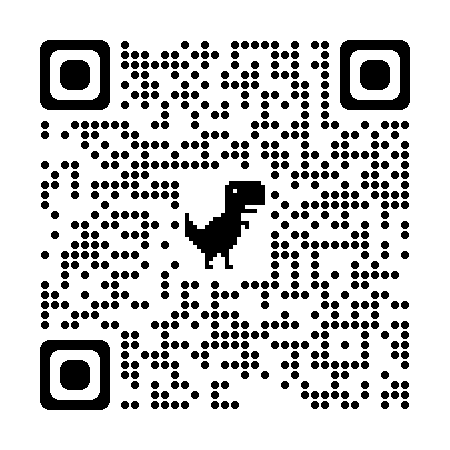
\includegraphics[width=0.4\linewidth]{figures/qrcode}
\end{figure*}


\endgroup
\newpage